\subsection{Aktivitätsdiagramm „Nothalt auslösen“}
\label{sec:aktivitaetsdiagramm_nothalt}
\begin{figure}[H]
    \centering
    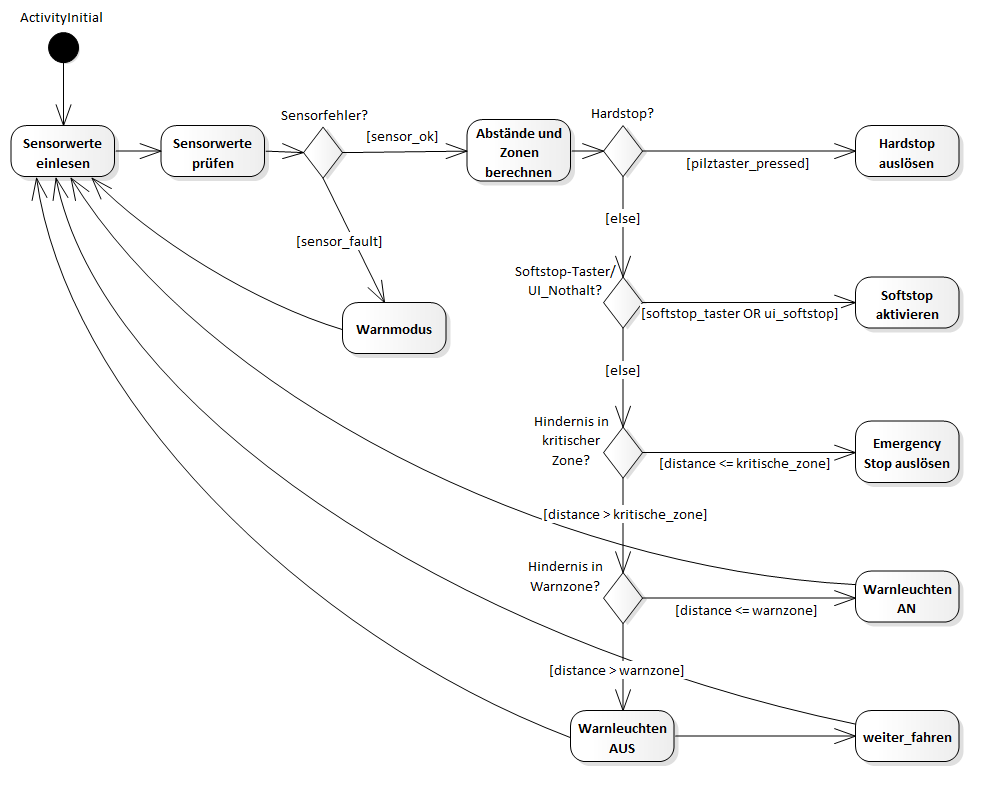
\includegraphics[width = \imglarge]{images/Nothalt_Aktivitätsdiagramm.png}
    \caption{Aktivitätsdiagramm „Nothalt auslösen“}
    \label{fig:aktivitaetsdiagramm_nothalt}
\end{figure}


\quad Das Aktivitätsdiagramm beschreibt den vollständigen Entscheidungsablauf des Nothaltesystems von der Erfassung der Sensordaten bis zur Auslösung sicherheitsrelevanter Reaktionen. Es zeigt den kontinuierlichen zyklischen Prozess, in dem Sensordaten geprüft, interpretierte Zonen bewertet und manuelle Eingaben des Operators berücksichtigt werden. 
Der Ablauf reflektiert die Priorisierung sicherheitskritischer Ereignisse (\ac{Hardstop} > \ac{Softstop} > automatischer \ac{E-Stop} > Warnung > Weiterfahren).

\subsection*{Initialer Zustand}

\quad Der Ablauf beginnt im ActivityInitial-Knoten und führt unmittelbar in die erste Aktivität:

\subsubsection*{1. Sensorwerte einlesen}

\quad Das System erfasst in regelmäßigen Intervallen die aktuellen Sensordaten:
\begin{itemize}
    \item LiDAR-Daten (2D/3D)
    \item Encoder-Werte
    \item eventuell weitere Sensordaten wie Zustandsmeldungen
\end{itemize}

\quad Alle Daten werden gesammelt und in den Verarbeitungspipeline überführt.

\subsubsection*{2. Sensorwerte prüfen}

\quad In einer Validierungsphase werden die eingelesenen Werte auf Plausibilität und Integrität geprüft.

\quad Typische Prüfungen:
\begin{itemize}
    \item Fehlmessungen
    \item Zeitstempelkonsistenz
    \item Kommunikationsfehler
    \item strukturelle Datenfehler (z.\,B.\ fehlerhafte PointCloud)
\end{itemize}

\subsubsection*{3. Entscheidung: Sensorfehler?}

\quad Der erste Entscheidungsknoten überprüft, ob ein sensor\_fault vorliegt.

\begin{description}
    \item[\texttt{[sensor\_fault]}] $\rightarrow$ Warnmodus aktivieren\\
    \quad Bei fehlerhafter Sensorik ist ein autonomer Weiterbetrieb nicht sicher möglich. Das System wechselt in einen abgesicherten Zustand (Warnmodus).
    \item[\texttt{[sensor\_ok]}] $\rightarrow$ Abstände und Zonen berechnen\\
    \quad Der normale Nothalt-Ablauf wird fortgesetzt.
\end{description}

\subsubsection*{4. Abstände und Zonen berechnen}

\quad Das System bestimmt aus den Sensordaten die aktuellen Abstände zu Objekten und ordnet diese den Gefahrenzonen zu:
\begin{itemize}
    \item kritische Zone (Sofortstopp erforderlich)
    \item Warnzone (nur optische Warnung, aber kein Stopp)
    \item freie Zone (keine Maßnahmen notwendig)
\end{itemize}

\subsubsection*{5. Entscheidung: \ac{Hardstop}?}

\quad Der nächste Entscheidungsknoten prüft, ob der Hardstop-Taster betätigt wurde:

\begin{description}
    \item[\texttt{[pilztaster\_pressed]}] $\rightarrow$ \ac{Hardstop} auslösen\\
    \quad Diese Aktion hat höchste Priorität. Sie führt unmittelbar zur Notabschaltung (Energie aus / Fahrzeugstop).
    \item[\texttt{[else]}] $\rightarrow$ Weiter zur \ac{Softstop}-Prüfung
\end{description}

\subsubsection*{6. Entscheidung: \ac{Softstop}-Taster oder UI-Nothalt?}

\quad Hier werden manuelle \ac{Softstop}-Signale ausgewertet:
\begin{itemize}
    \item physischer \ac{Softstop}-Taster
    \item \ac{Softstop}-Befehl über UI / RViz
\end{itemize}

\begin{description}
    \item[\texttt{[softstop\_taster OR ui\_softstop]}] $\rightarrow$ \ac{Softstop} aktivieren\\
    \quad Der \ac{Softstop} reduziert die Geschwindigkeit oder hält das Fahrzeug kontrolliert an.
    \item[\texttt{[else]}] $\rightarrow$ Weiter zur Hindernisbewertung
\end{description}

\subsubsection*{7. Entscheidung: Hindernis in kritischer Zone?}

\quad Wenn ein Objekt in der kritischen Zone erkannt wird:

\begin{description}
    \item[\texttt{[distance <= kritische\_zone]}] $\rightarrow$ Emergency Stop auslösen\\
    \quad Dies ist der automatische E-Stop, ausgelöst durch die Sensorik.
    \item[\texttt{[distance > kritische\_zone]}] $\rightarrow$ Weiter zur Warnzonenprüfung
\end{description}

\subsubsection*{8. Entscheidung: Hindernis in Warnzone?}

\quad Wenn ein Hindernis nicht kritisch, aber sicherheitsrelevant ist:

\begin{description}
    \item[\texttt{[distance <= warnzone]}] $\rightarrow$ Warnleuchten AN\\
    \quad Das Fahrzeug fährt weiter, aber signalisiert eine Gefahrenlage.
    \item[\texttt{[distance > warnzone]}] $\rightarrow$ Warnleuchten AUS $\rightarrow$ weiter\_fahren
\end{description}

\subsubsection*{9. Weiterfahren}

\quad Wenn weder \ac{Hardstop}, \ac{Softstop}, \ac{E-Stop} noch Warnsignale notwendig sind, 
bleibt das Fahrzeug im normalen Fahrbetrieb und der Zyklus beginnt erneut.
